\chapter{Consistency Study of Adversarial loss}
\label{chap:calibration}

\minitoc
\textbf{Disclaimer: This section is still an unachieved work}

In this section we assume a binary classification task, i.e. an output space $\mathcal{Y}=\{-1,+1\}$. W extend the notion of loss functions to general cost functions.  A cost function is a function $\loss:\mathcal{X}\times\mathcal{Y}\times \mathcal{F}(\mathcal{X})\to \mathbb{R}$ such that $\loss(\cdot,\cdot,f)$ is universally measurable for all $f\in\mathcal{F}(\mathcal{X})$. We will denote $\mathcal{R}_{\loss}$ the risk associated with a loss $\loss$. 


\section{Loss Consistency in Classification}

\subsection{Consistency in Standard Classification}
In a standard classification setting,  given $(x,y)$, we recall  the classification loss is defined as:
\begin{align*}
    \loss_{0/1}(x,y,f) = \mathbf{1}_{y\sign(f(x))\leq 0}
\end{align*}
In the literature the notion of consistency with regards to the $0/1$ loss is defined as follows.
\begin{definition}[Classification Consistency]
A cost function $\loss$ is said to be consistent with respect to $0/1$ loss for a a probability distribution $\PP\in\mathcal{M}_1^+(\mathcal{X}\times\mathcal{Y})$ if and only if for all sequences $(f_n)_n $ of measurable functions:
\begin{align}
    \mathcal{R}_{\loss}(f_n)\to \mathcal{R}_{\loss}^\star\implies\mathcal{R}_{0/1}(f_n)\to \mathcal{R}_{0/1}^\star
\end{align}
\end{definition}


\paragraph{Standard results in classification.} Previous literature have focused, in standard classification, on margin losses, and it is defined as follows.

\begin{definition}[Margin loss] We say a loss $\loss$ is a margin loss if there exists a measurable function $\phi:\mathbb{R}\to\mathbb{R}_+$, such that for all $x\in\mathcal{X}$, $y\in\mathcal{Y}$, $f:\mathcal{X}\to\mathbb{R}$ a measurable function,
$$\loss(x,y,f)=\phi(yf(x))$$
\end{definition}
Without loss of generality, we will denote $\mathcal{R}_\phi$ the risk associated with a margin loss. Standard classification consistency highly relies on the fact that given a loss, the minimization can be made pointwisely, independently from the considered distribution $\PP$. The notion of consistency exactly matches with the notion of calibration, defined as follows:
\begin{definition}[Classification Calibration] A margin loss $\phi$ is said to be classification-calibrated if for all $\eta\in[0,1]$, $\eta\neq \frac12$:
\begin{align*}
    H(\eta)>H^-(\eta)
\end{align*}
where $H(\eta):=\inf_{\alpha\in\RR}C_\eta(\alpha)$,  $H^-(\eta) = \inf_{\alpha,~\alpha(2\eta-1)\leq0}C_\eta(\alpha)$ and $C_\eta(\alpha):=\eta\phi(\alpha)+(1-\eta)\phi(-\alpha)$.
\end{definition}

\cite{bartlett2006convexity} and \cite{steinwart2007compare} show that consistency and calibration are equivalent notions in standard classification.

\begin{thm} In standard calibration, a margin loss $\phi$ is consistent with regards to classification loss if and only if $\phi$ is classification calibrated. 
\end{thm}

In particular, one can state the following results on convex margin losses.
\begin{thm} Let $\phi$ be a convex margin differentiable in $0$. $\phi$ is consistent with regards to  classification loss if and only if $\phi'(0)<0$.
\end{thm}
\paragraph{What is the good 0/1 loss?}
In this paragraph, we precise why this $0/1$ loss is used in consistency/calibration study. Let $f:\mathcal{X}\to\mathbb{R}$ be a measurable function. In the literature,  we generally find three ways for defining the $0/1$ loss:
\begin{itemize}
    \item $\loss_{\leq}(x,y,f)=\mathbf{1}_{yf(x)\leq 0}$, the loss that penalizes indecision.
    \item $\loss_{<}(x,y,f)=\mathbf{1}_{yf(x)< 0}$, the loss that encourages indecision.
    \item $\loss_{0/1}(x,y,f)=\mathbf{1}_{y\text{sign}(f(x))\leq 0}$, with a sign convention ($sign(0) = 1$ for instance).
\end{itemize}

The original results from~\citep{bartlett2006convexity,steinwart2007compare} tackles the problem of the consistency with respect to the latter one. We can even remark that usual consistency results stated in the two previous papers are false for the two first losses, as shown in the following simple counterexample.

\begin{counterexample*}
Let $\PP$ defined as follows: $\PP(Y=-1)=\PP(Y=1)=\frac12$, and $\PP(X=0\mid Y)=1$. Let $\phi:\mathbb{R}\to\mathbb{R}$ be a margin  loss. The $\phi$-risk minimization problem writes $\inf_{\alpha} \frac{1}{2} (\phi(\alpha)+\phi(-\alpha))$. For a convex margin loss $\phi$ the optimum is attained in $\alpha=0$. 
\begin{enumerate}
    \item $f_n:x\mapsto 0$ is a minimizing sequence for the $\phi$-risk. However $R_{\loss_{\leq}}(f_n)=1$ for all $n$ and $R_{\loss_{\leq}}^*=\frac{1}{2}$. Then we deduce that no convex margin based loss can be calibrated for $\loss_{\leq}$.
    \item $f_n:x\mapsto \frac{1}{n}$ is a minimizing sequence for the $\phi$-risk. However $R_{\loss_{<}}(f_n)=1/2$ for all $n$ and $R_{\loss_{<}}^*=0$. Then we deduce that no convex margin based loss can be calibrated for $\loss_{<}$.
\end{enumerate}

\end{counterexample*}



\subsection{Consistency in adversarial setting}


Consistency in standard classification is studied with respect to the cost $\loss_{0/1}(x,y,f)=\mathbf{1}_{y\text{sign}(f(x))\leq 0}$. In the adversarial setting, the natural loss to consider then is  $$\loss_{0/1,\varepsilon}(x,y,f)=\sup_{x'\in B_\varepsilon(x)}\mathbf{1}_{y\text{sign}(f(x'))\leq 0}$$ 
with a sign convention (e.g. $sign(0)=1$). Otherwise, when $\varepsilon=0$, the consistency results would be wrong as stated in the previous counterexample. Previous works~\citep{pmlr-v125-bao20a,awasthi2021calibration,awasthi2021finer} focused on the loss $\sup_{x'\in B_\varepsilon(x)}\mathbf{1}_{yf(x')\leq 0}$ that consequently lead to misleading results because not compatible with standard classification when $\varepsilon=0$. We define the notion of consistency with regards to adversarial $0/1$ loss as follows.
\begin{definition}[Adversarial Consistency]
A cost function $\loss$ is said to be consistent with respect to $0/1$ loss for a distribution  $\PP\in\mathcal{M}_1^+(\mathcal{X}\times\mathcal{Y})$ if and only if for all sequences $(f_n)_n $ of measurable functions:
\begin{align}
    \mathcal{R}_{\loss}(f_n)\to \mathcal{R}_{\loss}^\star\implies\mathcal{R}_{0/1}^\varepsilon(f_n)\to \mathcal{R}_{0/1}^{\varepsilon,\star}
\end{align}
\end{definition}

\paragraph{Calibration in adversarial classification} One need to note that the notion of calibration in the adversarial setting is misleading.  

TODO.



Hence, one need to focus specifically on the notion of consistency in the adversarial setting. In the next section, we prove some results on adversarial consistency.

\section{Adversarial Consistency Results}

\subsection{Convex Losses are not Consistent}
Following the work on standard classification, natural candidate losses for adversarial consistency would be suprema of standardly calibrared margin losses:

$$\loss(x,y,f)=\sup_{x', d(x,x')\leq\varepsilon}\phi(yf(x))$$
including a wide range of  convex functions $\phi$. Next theorem shows the counter-intuitive result that no calibrated convex loss can define a consistent loss for adversarial classification
\begin{prop}
Let $\phi$ be a convex classification-calibrated margin loss (i.e. $\phi'(0) <0$). In $\RR$, for any $\varepsilon > 0$, there exists a distribution $\PP$ such that $x\to\sup_{x', d(x,x')\leq\varepsilon}\phi(yf(x))$ is not consistent for $\PP$ with regards to $\loss_{0/1,\varepsilon}$.
\end{prop}

\begin{proof}

Let $\epsilon$ > 0. We will construct a distribution $\mathcal{D}$ and a sequence of classifier $h_n$ so that the $\phi$-risk converges toward the optimal, while the $0-1$ loss remains constant at a non-optimal value.

\paragraph{}Let a such that $\epsilon < a < 2 \epsilon$. We define D by :
\[
\left\{ \begin{array}{ll}
\mathbb{P}(Y=1, X=0) = \frac{1}{2} & \\
\mathbb{P}(Y=-1, X=-a) = \frac{1}{4} & \\
\mathbb{P}(Y=-1, X=a) = \frac{1}{4} & \\
\mathbb{P}(X, Y) = 0 & \mbox{otherwise.} \\
\end{array} \right.
\]

Since $\phi$ is classification-calibrated, it is either non-increasing, or it has a minimum, attained on a point $u>0$. Let us consider both cases :

\paragraph{First case : $\phi$ non-increasing}

We define $Z_1 = [-\epsilon, -a + \epsilon]$ and $Z_2 = [a-\epsilon, \epsilon]$, the zones that can be attacked by two points at once.
Let us then define : 
\[
\forall x \in \mathbb{R}, h_n(x) = \left\{ \begin{array}{ll}
\frac{1}{n} & \mbox{if } x \in Z_1 \\
-1/n & \mbox{if } x \in Z_2 \\
1 & \mbox{if }x \in [-a+\epsilon, a-\epsilon] \\
-1 & \mbox{otherwise} \\
\end{array} \right.
\]

\begin{figure}
    \centering
    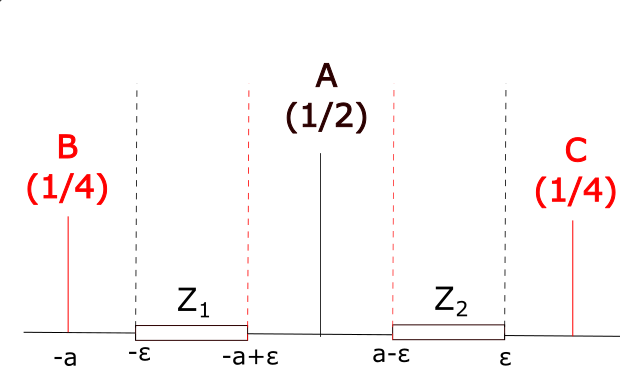
\includegraphics[scale=0.6]{sections/3_calibration/images/example.png}
    \caption{The distribution we use as a counter-example. For the $0-1$ loss, there are two optimal classifiers, putting either both $Z_1$ and $Z_2$ to $1$ (and saving point A), or both to $-1$ (saving points B and C). With convex surrogate losses however, the optimal is to bring values in both $Z_1$ and $Z_2$ to zero, which can be done while maintaining opposite signs on $Z_1$ and $Z_2$, and so ensuring the loss of both A and one of B and C for the $0-1$ loss. }
    \label{fig:my_label}
\end{figure}


Since the central point and the point $x=-a$ are attackable, but not the point $x=a$, we have $\mathbb{E}_{(x,y)\sim \mathcal{D}}\left[ \sup\limits_{z \in \mathcal{B}(x,\epsilon)} l_{0/1}(y,h_n(z))\right] = \frac{3}{4}$, which is worse than the constant classifier h=1, which gives a score of $\frac{1}{2}$. So $h_n$ is not a minimizing sequence for the $0-1$ loss.

Let us now show that $h_n$ is a minimizing sequence for the loss $\phi$ under attack, which will be proof of the non-consistency.

\begin{align*}
    \mathbb{E}_{(x,y)\sim \mathcal{D}}\left[ \sup\limits_{z \in \mathcal{B}(x,\epsilon)} \phi(y*h_n(z))\right] &= \frac{1}{2} \phi(\frac{-1}{n}) +\frac{1}{4}\phi(\frac{1}{n}) + \frac{1}{4}\phi(\frac{1}{n})\\
    &=\frac{1}{2}\phi(\frac{-1}{n}) + \frac{1}{2}\phi(\frac{1}{n}) \\
    &\underset{n\to +\infty}{\longrightarrow}\phi(0)
\end{align*}

We now need to show that $\phi(0)$ is a lower bound of the optimal adversarial risk for the loss $\phi$.
Let h be any  classifier. We define :
\begin{align*}
b &= \inf\limits_{z \in \left[ -a + \epsilon, a- \epsilon \right]} h(z) \\
c &= \sup\limits_{z \in \left[ -a - \epsilon, -\epsilon \right]} h(z) \\
d &= \sup\limits_{z \in \left[\epsilon, a + \epsilon \right]} h(z) \\
m_i &= \inf\limits_{z \in \mathcal{Z}_i} h(z) \mbox{  for  }i \in \left\{ 1,2\right\} \\
M_i &= \sup\limits_{z \in \mathcal{Z}_i} h(z) \mbox{  for  }i \in \left\{ 1,2\right\} \\
m &= \min(m_1,m_2)
\end{align*}

We then have :

\begin{align*}
    \mathbb{E}_{(x,y)\sim \mathcal{D}}\left[ \sup\limits_{z \in \mathcal{B}(x,\epsilon)} \phi(y*h_n(z))\right] &= \frac{1}{2} \sup\limits_{ z \in \left[ -\epsilon, \epsilon \right]} \phi(h(z))
            + \frac{1}{4}\sup\limits_{z \in \left[ -a-\epsilon, -a+\epsilon \right]} \phi(-h(z)) 
            + \frac{1}{4}\sup\limits_{z \in \left[ a-\epsilon, a+\epsilon \right]} \phi(-h(z)) \\
    &= \frac{1}{2} \max \left[ \sup\limits_{ z \in \left[ -a+\epsilon, a-\epsilon \right]} \phi(h(z)), \sup\limits_{ z \in \mathcal{Z}_1} \phi(h(z)), \sup\limits_{ z \in \mathcal{Z}_2} \phi(h(z)) \right] \\
    &+ \frac{1}{4} \max \left[ \sup\limits_{ z \in \left[ -a-\epsilon, -\epsilon \right]} \phi(-h(z)), \sup\limits_{ z \in \mathcal{Z}_1} \phi(-h(z)) \right] \\
    &+ \frac{1}{4} \max \left[ \sup\limits_{ z \in \left[ \epsilon, a+\epsilon \right]} \phi(-h(z)), \sup\limits_{ z \in \mathcal{Z}_2} \phi(-h(z)) \right] \\
    &= \frac{1}{2} \max \left[ \phi(b), \phi(m_1), \phi(m_2) \right]
    + \frac{1}{4} \max \left[ \phi(-M_1), \phi(-c) \right] \\
    &+ \frac{1}{4} \max \left[ \phi(-M_2), \phi(-c) \right] \\
    &\geq \frac{1}{2} \max \left[\phi(m_1), \phi(m_2) \right] + \frac{1}{4}\phi(-M_1) + \frac{1}{4}\phi(-M_2) \\
    &\geq \frac{1}{2} \phi(m) + \frac{1}{4}\phi(-m) + \frac{1}{4}\phi(-m) \\
    &\geq \phi(0)
\end{align*}

Hence the result.
\end{proof}


\subsection{Realisable case}
In this realisable case, i.e. $\mathcal{R}^{\varepsilon}_{0/1} = 0$, results about standard classification consistency still hold.
\begin{prop}
Let $\PP$ be a Borel probability distribution over $\mathcal{X}\times\mathcal{Y}$ such that $\mathcal{R}^{\varepsilon}_{0/1} = 0$. Then, let $\phi$ be a standard classification calibrated margin-based loss. Then $\Tilde{\phi}:(x,y,f)\mapsto\sup_{x'\in B_\varepsilon(x)}\phi(yf(x'))$ is adversarially consistent at level $\varepsilon$.
\end{prop}

\begin{proof}
Coming soon
\end{proof}